\chapter{相關應用}

\section{電子鼻}
\begin{enumerate}
	\item 
	Fast GC Analyzer 電子鼻 (簡稱 zNose® ,Electronic Sensor Technology),
	使用 Tenax 為吸附劑,待吸附氣分子後,利用熱脫附裝置,使氣味分子快速進入層析系統,
	於 10-20 秒內完成分離後,以表面聲波共振(surface acoustic wave resonator) 偵測,
	記錄各分離物種之滯留時間與信號強度,繪製嗅覺影像圖,與已知的氣味嗅覺影像圖資料比對,
	得知氣味的種類。(取自參考文獻 1 - 異味氣體之偵測)
	\begin{figure}[H]
		\centering
		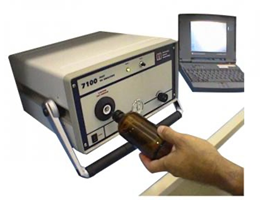
\includegraphics[width=0.5\textwidth]{../../pic/nose.png}
	\end{figure}
\end{enumerate}

\section{Alpla MOS}
Alpha MOS 由 6 個氣體感測器陣列所組成的 RQBOX 模組氣體監測系統,具有無線訊號傳輸裝置,
模組內的無線傳輸裝置可提供即時的遠端訊號傳輸,實際測試的結果顯示,其傳輸距離可達三百多公尺遠。
藉由連接有訊號接收器的電腦,可以提供遠端遙控即時空氣品質監測的功能。(取自參考文獻 1 - 異味氣體之偵測)

\section{感知比較實驗}
進行人的嗅覺系統對於臭氣的感知比較實驗(三點比較式嗅袋法)- 人體嗅覺是否能察覺有害氣體。(取自參考文獻 1 - 異味氣體之偵測)

\section{氣味感測器實例應用}
(取自參考文獻 1 - 異味氣體之偵測)\\
	\subsection{油管漏油事件}
	輸油管不論是遭受意外或人為蓄意破壞,漏油所影響的面積和環境污染程度最為嚴重。
	應用電子鼻分析結果。顯示整合現場快速判定未知樣品之電子鼻分析技術,協助取得代表性樣品,
	藉由 GC-MS 確認分析,同時達到緊急應變處置,降低災害至最低。
	\subsection{辦公大樓室內空氣異味事件}
	2002 年 11 月前往內疑有異味且地面有異物之辦公大樓,進行採樣檢測以了解可能原因。
	\subsection{羊乳摻牛乳事件}
	使用儀器分析羊乳中是否有牛乳摻假,多利用羊、牛乳中之脂肪酸或蛋白質(酪蛋白或乳清蛋白)組分之差異。
	使用電子鼻具有檢測時間短、檢測方法簡單、操作方法容易等優點。